\documentclass[a4paper,11pt]{article}
\usepackage[T1]{fontenc}
\usepackage[utf8]{inputenc}
\usepackage{amsmath}
\usepackage{siunitx}
\usepackage{tikz}
\usepackage[margin=2.5cm]{geometry}
\usetikzlibrary{arrows.meta}

\title{ATCG I Sheet R04 Solution}
\author{
\large Kamran Moradnejad (3099229) \\
\large Pranav Yadav (50327698) \\
\large Saransh Jain (50262919)
}
\date{May 8, 2026}

\begin{document}
\maketitle

\section*{Assignment 2: Refraction in Wedge}
The wedge is a $45^\circ$-$45^\circ$-$90^\circ$ prism surrounded by air with refractive index
\[
n_a = 1.
\]
The laser hits the left face perpendicularly, so at the first interface the transmitted ray continues without deflection. Inside the wedge the ray therefore travels horizontally and meets the slanted faces with an incidence angle of
\[
\theta_i = 45^\circ
\]
measured to the surface normal.

\subsection*{a) Wedge with $n_w = \sqrt{3/2} \approx 1.225$}
The critical angle for a transition from wedge material to air is
\[
\theta_c = \arcsin\left(\frac{n_a}{n_w}\right)
= \arcsin\left(\frac{1}{\sqrt{3/2}}\right)
\approx 54.74^\circ.
\]
Since
\[
45^\circ < \theta_c,
\]
there is no total internal reflection at the slanted faces.

Snell's law at a slanted face gives
\[
n_w \sin\theta_i = n_a \sin\theta_t
\]
and therefore
\[
\sin\theta_t = \sqrt{\frac{3}{2}}\sin 45^\circ
= \sqrt{\frac{3}{2}}\cdot \frac{\sqrt{2}}{2}
= \frac{\sqrt{3}}{2}.
\]
Hence
\[
\theta_t = 60^\circ.
\]
So every hit on a slanted face produces
\begin{itemize}
    \item one transmitted ray leaving the wedge at $60^\circ$ to the face normal,
    \item one reflected ray remaining inside the wedge and hitting the opposite slanted face again at $45^\circ$.
\end{itemize}

\begin{center}
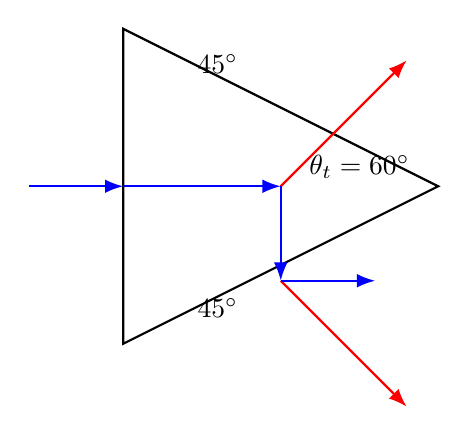
\begin{tikzpicture}[scale=1.0, >=Latex]
    \draw[thick] (0,0) -- (0,4) -- (4,2) -- cycle;
    \draw[->, blue, thick] (-1.2,2) -- (0,2);
    \draw[->, blue, thick] (0,2) -- (2,2);
    \draw[->, red, thick] (2,2) -- (3.6,3.6);
    \draw[->, blue, thick] (2,2) -- (2,0.8);
    \draw[->, red, thick] (2,0.8) -- (3.6,-0.8);
    \draw[->, blue, thick] (2,0.8) -- (3.2,0.8);
    \node at (1.2,3.55) {$45^\circ$};
    \node at (1.2,0.45) {$45^\circ$};
    \node at (3.0,2.25) {$\theta_t = 60^\circ$};
\end{tikzpicture}
\end{center}

\subsection*{b) Wedge with $n'_w = 5$}
Now the critical angle becomes
\[
\theta'_c = \arcsin\left(\frac{1}{5}\right) \approx 11.54^\circ.
\]
Since
\[
45^\circ > \theta'_c,
\]
every hit on a slanted face undergoes total internal reflection. Therefore the internal ray is trapped between the two slanted faces and no refracted ray leaves through them.

\begin{center}
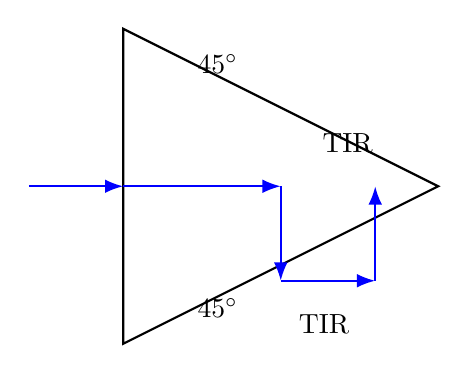
\begin{tikzpicture}[scale=1.0, >=Latex]
    \draw[thick] (0,0) -- (0,4) -- (4,2) -- cycle;
    \draw[->, blue, thick] (-1.2,2) -- (0,2);
    \draw[->, blue, thick] (0,2) -- (2,2);
    \draw[->, blue, thick] (2,2) -- (2,0.8);
    \draw[->, blue, thick] (2,0.8) -- (3.2,0.8);
    \draw[->, blue, thick] (3.2,0.8) -- (3.2,2.0);
    \node at (1.2,3.55) {$45^\circ$};
    \node at (1.2,0.45) {$45^\circ$};
    \node at (2.85,2.55) {TIR};
    \node at (2.55,0.25) {TIR};
\end{tikzpicture}
\end{center}

\subsection*{c) Difference between the two scenarios}
For $n_w = \sqrt{3/2}$ the angle of incidence at the slanted faces is smaller than the critical angle, so the ray can leave the wedge through those faces. For $n'_w = 5$ the critical angle is much smaller than $45^\circ$, so the slanted faces show total internal reflection and the light remains trapped inside the prism apart from the initial reflection at the entrance face.

\subsection*{d) Smallest refractive index with the same behavior as $n'_w$}
To get the same qualitative result as in part b), the incidence angle at the slanted faces must be at least the critical angle. The threshold case is
\[
\theta_c = 45^\circ.
\]
Thus
\[
\arcsin\left(\frac{1}{\hat n_w}\right) = 45^\circ
\]
which implies
\[
\frac{1}{\hat n_w} = \sin 45^\circ = \frac{\sqrt{2}}{2}.
\]
Therefore
\[
\boxed{\hat n_w = \sqrt{2} \approx 1.4142.}
\]

\section*{Assignment 3: Refraction in Slab}
The incident angle is given as $50^\circ$ measured to the surface. Therefore the angle to the surface normal is
\[
\theta_i = 90^\circ - 50^\circ = 40^\circ.
\]
The refractive indices are
\[
n_a = 1,
\qquad
n_g = 1.5.
\]

\subsection*{a) Light paths up to 6 reflections/refractions}
Snell's law at the first interface gives
\[
n_a \sin\theta_i = n_g \sin\theta_t
\]
and thus
\[
\sin\theta_t = \frac{1}{1.5}\sin 40^\circ \approx 0.4285.
\]
So the angle inside the slab is
\[
\theta_t \approx 25.37^\circ
\]
to the surface normal.

The first six paths are:
\begin{itemize}
    \item immediate reflection at the top interface,
    \item first transmission through the slab and exit at the bottom,
    \item one internal reflection and exit at the top,
    \item two internal reflections and exit at the bottom,
    \item three internal reflections and exit at the top,
    \item four internal reflections and exit at the bottom.
\end{itemize}

\begin{center}
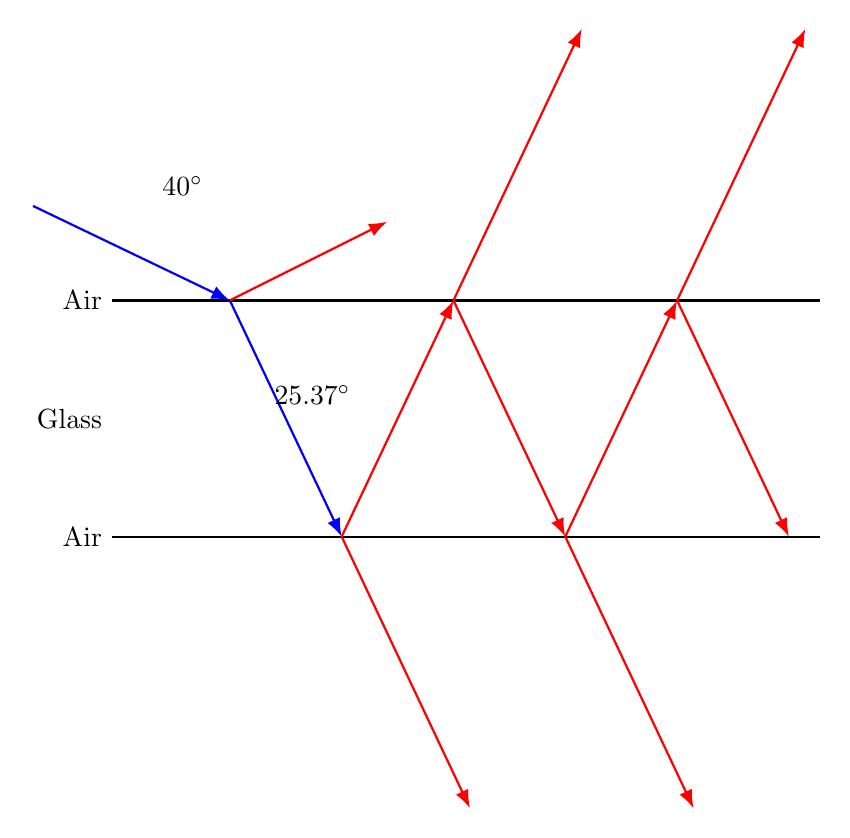
\begin{tikzpicture}[scale=1.0, >=Latex]
    \draw[thick] (-0.5,3) -- (8.5,3);
    \draw[thick] (-0.5,0) -- (8.5,0);
    \node[left] at (-0.5,3) {Air};
    \node[left] at (-0.5,1.5) {Glass};
    \node[left] at (-0.5,0) {Air};

    \draw[->, blue, thick] (-1.5,4.2) -- (1.0,3.0);
    \draw[->, red, thick] (1.0,3.0) -- (3.0,4.0);

    \draw[->, blue, thick] (1.0,3.0) -- (2.42,0.0);
    \draw[->, red, thick] (2.42,0.0) -- (3.84,3.0);
    \draw[->, red, thick] (2.42,0.0) -- (4.05,-3.45);
    \draw[->, red, thick] (3.84,3.0) -- (5.26,0.0);
    \draw[->, red, thick] (3.84,3.0) -- (5.47,6.45);
    \draw[->, red, thick] (5.26,0.0) -- (6.68,3.0);
    \draw[->, red, thick] (5.26,0.0) -- (6.89,-3.45);
    \draw[->, red, thick] (6.68,3.0) -- (8.10,0.0);
    \draw[->, red, thick] (6.68,3.0) -- (8.31,6.45);

    \node at (0.4,4.45) {$40^\circ$};
    \node at (2.05,1.8) {$25.37^\circ$};
\end{tikzpicture}
\end{center}

\subsection*{b) Light fractions emitted to top and bottom}
For unpolarized light we average the s- and p-polarized Fresnel reflectances. At the air-glass interface:
\[
R_s = \left(\frac{n_a\cos\theta_i - n_g\cos\theta_t}{n_a\cos\theta_i + n_g\cos\theta_t}\right)^2,
\qquad
R_p = \left(\frac{n_a\cos\theta_t - n_g\cos\theta_i}{n_a\cos\theta_t + n_g\cos\theta_i}\right)^2.
\]
Numerically, with $\theta_i = 40^\circ$ and $\theta_t \approx 25.37^\circ$,
\[
R = \frac{R_s + R_p}{2} \approx 0.0457336,
\qquad
T = 1 - R \approx 0.9542664.
\]

Because the slab interfaces are parallel, the same reflectance and transmittance apply at each internal hit. The total fraction leaving through the bottom is therefore
\[
L_{\text{bottom}} = T^2 \left(1 + R^2 + R^4 + \cdots\right)
= \frac{T^2}{1-R^2}.
\]
Numerically,
\[
L_{\text{bottom}} \approx \frac{0.9542664^2}{1-0.0457336^2}
\approx 0.9125329.
\]

The total fraction leaving through the top is the direct top reflection plus all later exits after an odd number of internal reflections:
\[
L_{\text{top}} = R + T^2R\left(1 + R^2 + R^4 + \cdots\right)
= R + \frac{T^2R}{1-R^2}.
\]
Numerically,
\[
L_{\text{top}} \approx 0.0457336 + \frac{0.9542664^2 \cdot 0.0457336}{1-0.0457336^2}
\approx 0.0874671.
\]

As a consistency check,
\[
L_{\text{top}} + L_{\text{bottom}} \approx 0.0874671 + 0.9125329 = 1.
\]

Hence,
\[
\boxed{L_{\text{top}} \approx 0.08747}
\]
and
\[
\boxed{L_{\text{bottom}} \approx 0.91253.}
\]

\end{document}
